% !TEX root =  ../supplementary.tex
\section{Personalized Schedules for the Demonstration Patients from PRIAS.}
\label{sec : demo_3174_2340}

In this section we demonstrate the application of personalized schedules on patients from PRIAS study. In Section \ref{subsec : demo_prias_pers_schedule} of the main manuscript we demonstrated personalized schedules for the first demonstration patient. Here we demonstrate them for the remaining two patients.

The evolution of PSA, repeat biopsy history and proposed times of biopsies for the second demonstration patient are shown in the top right and top left panels of Web Figure \ref{fig : prias_demo_pid_3174}. It can be seen that the schedule of biopsy based on expected time of GR adjusts the times of biopsy according to the rise in hazard, which increases due to steep rise in $\log_2 \mbox{PSA}$ velocity. More specifically, at year two the proposed biopsy time is 12.36 years whereas at year four it decreases to 3.94 years. On average, a biopsy scheduled using expected time of GR at year two should have a larger offset $O^S_j$ compared to the same at year four. This is because the standard deviation of $g(T^*_j)$, given by $\mbox{SD}_g(T^*_j) = \sqrt{\mbox{var}_g(T^*_j)}$, is slightly lower at year four as shown in the bottom left panel of Web Figure \ref{fig : prias_demo_pid_3174}. As for the schedules based on dynamic risk of GR, the threshold $\kappa$ was automatically chosen using $\mbox{F}_1$ score, and was estimated to be between 1 and 0.9 at all time points. This value of $\kappa$ corresponds to a time very close to the time of latest biopsy ($t=0$). Hence the biopsies are scheduled much earlier than those based on expected time of GR.

\begin{figure}
\centerline{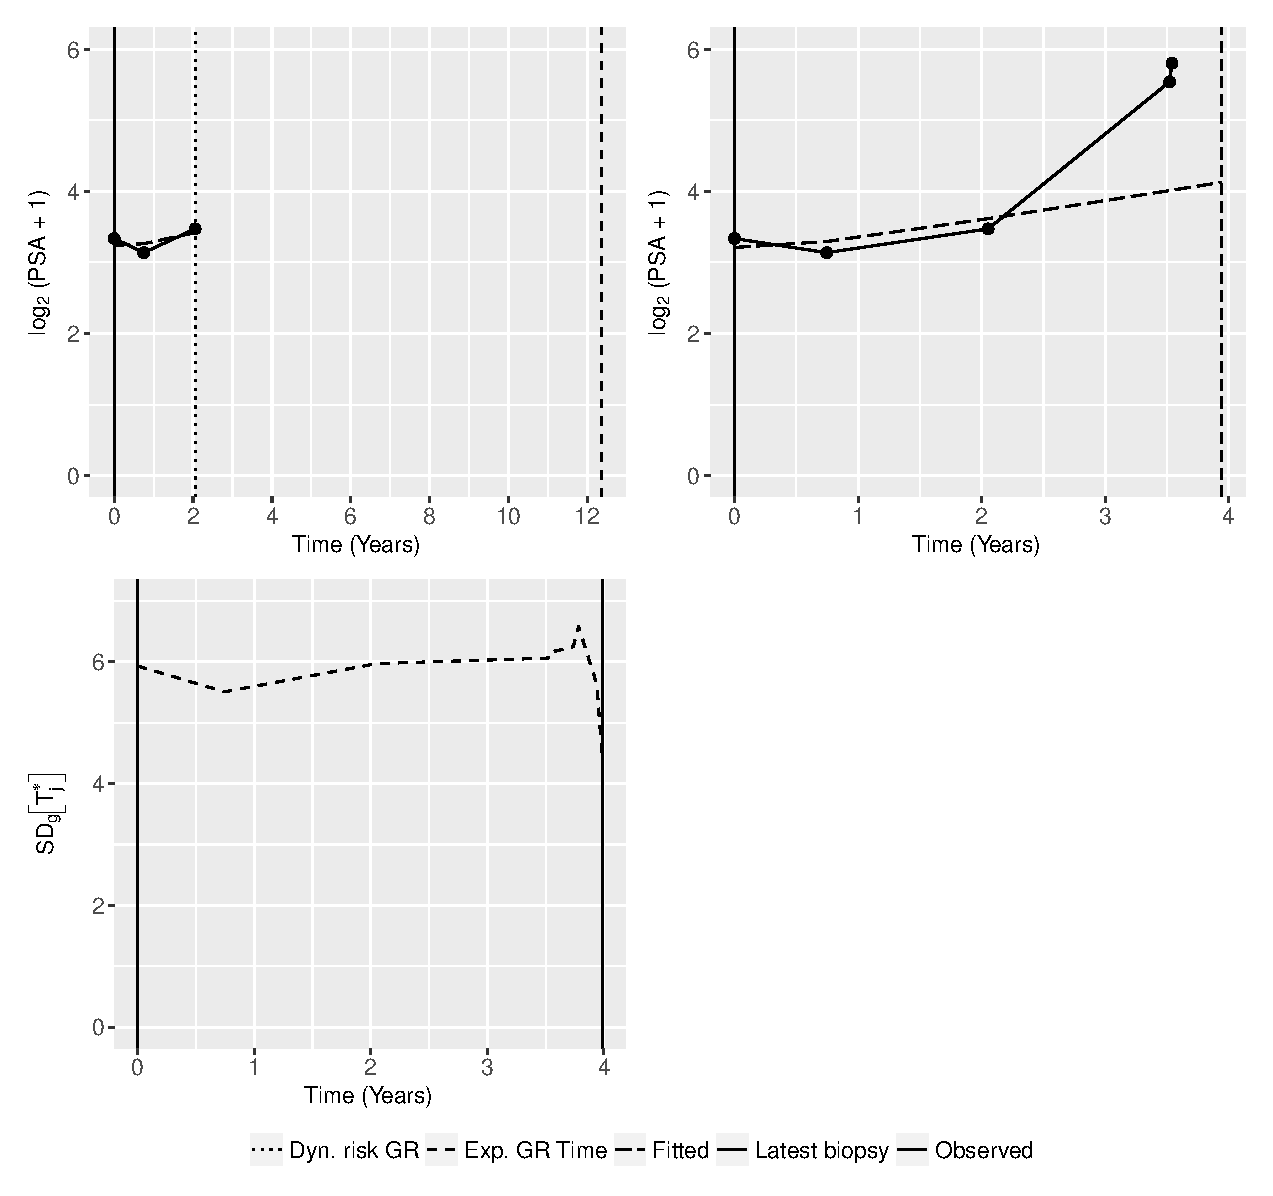
\includegraphics[width=\columnwidth]{images/prias_demo/case_3174_t3_log2psa_plus1.eps}}
\caption{Top panel: Fitted versus observed $\log_2 (\mbox{PSA} + 1)$ profile, history of repeat biopsies and corresponding personalized schedules for the second demonstration patient. Bottom Panel: History of repeat biopsies and standard deviation $\mbox{SD}_g(T^*_j) = \sqrt{\mbox{var}_g(T^*_j)}$ of the posterior predictive distribution of time of GR over time for the second demonstration patient.}
\label{fig : prias_demo_pid_3174}
\end{figure}

\clearpage

The third demonstration patient presents a case where information from PSA levels and repeat biopsies is not in concordance with each other. In Web Figure \ref{web_fig : prias_demo_pid_2340} we can see that the PSA for this patient increased by 100\% between year two and year 3.2. If only information from PSA is considered, then we can see that proposed time of biopsy based on expected time of GR is preponed from 14.26 to 13.56 years during this period. However, if we also take into account the negative result from the repeat biopsy at year 2.5, then the proposed time of biopsy is postponed from 14.26 years to 15.15 years. Thus more weight is given to a recent negative biopsy result than PSA, which is in accordance with the clinical practice. The proposed time of biopsy based on dynamic risk of GR is also postponed from 2.27 to 3.55 years in light of the negative biopsy result.

\begin{figure}
\centerline{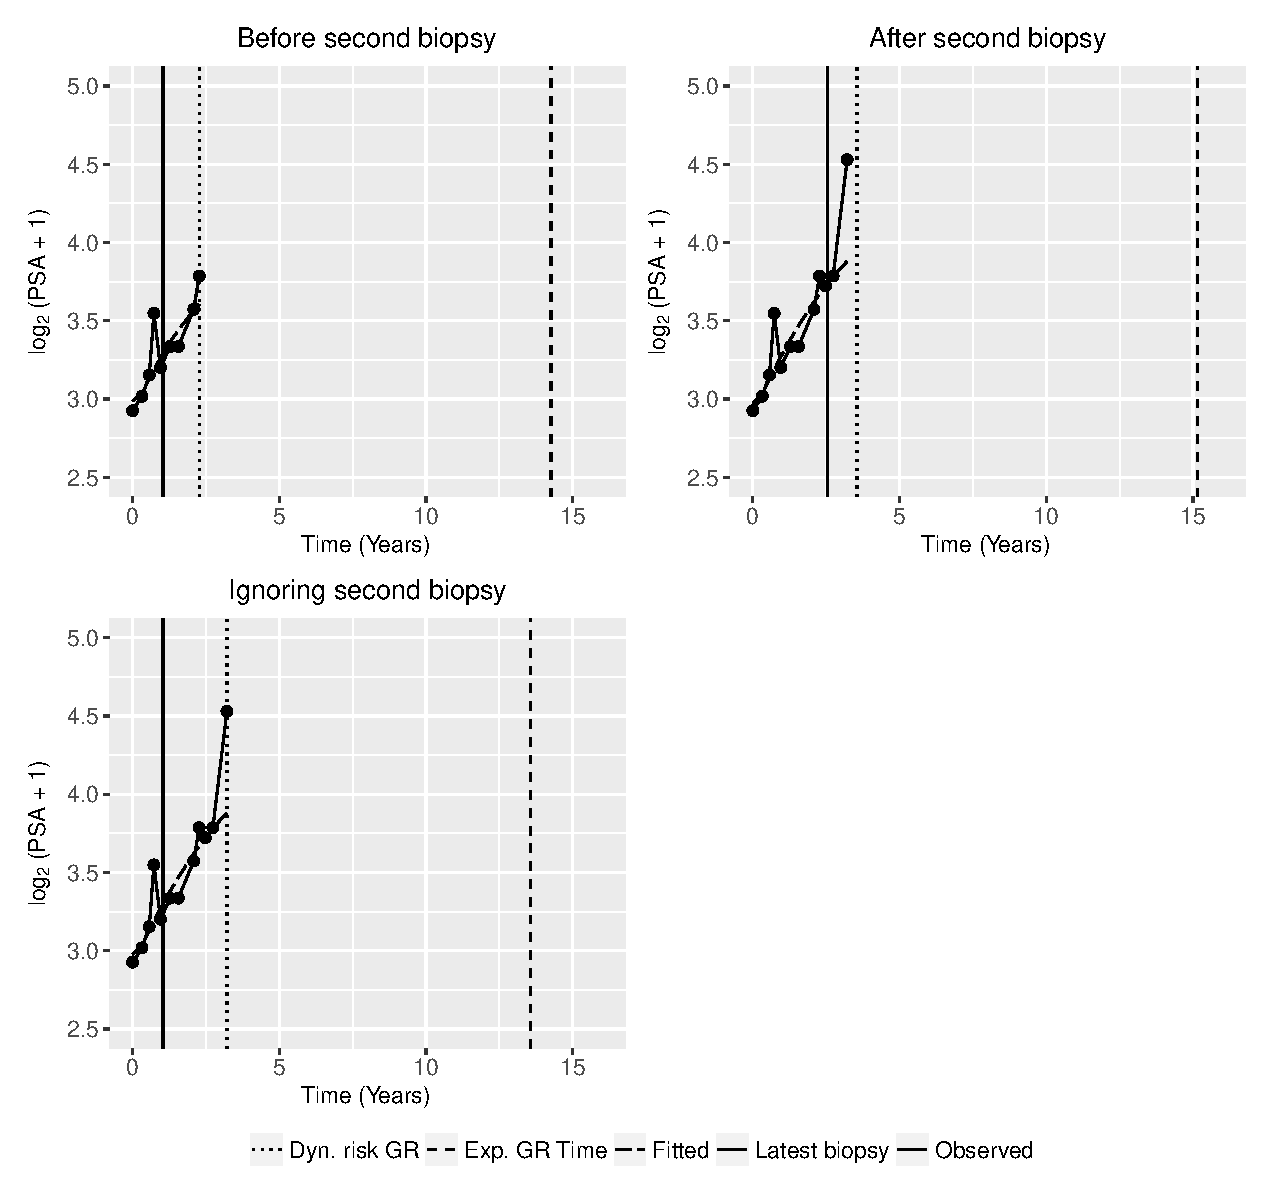
\includegraphics[width=\columnwidth]{images/prias_demo/case_2340_t3_log2psa_plus1.eps}}
\caption{Fitted versus observed $\log_2 (\mbox{PSA} +1)$ profile, history of repeat biopsies and corresponding personalized schedules for the third demonstration patient.}
\label{web_fig : prias_demo_pid_2340}
\end{figure}